\documentclass[10pt,aspectratio=43]{beamer}
\usepackage{fsu2017}
% the aspactratio defines the foramt
% default is 43 (4:3, 128mm:96mm), alternatives are
% 32 (3:2, 135mm:90mm)
% 54 (5:4, 125mm:100mm)
% 149 (14:9, 14cm:9cm)
% 169 (16:9, 16cm:9cm)
% 1610 (16:10, 16cm:10cm)
% 141 (1.41:1, 148.5mm:105mm, ratio of DinA)

\usepackage{color}

% graphic settings
\usepackage{graphicx}
\usepackage{tikz}
\usepackage{pgfplots}
\usepackage{accents}
\usetikzlibrary{arrows.meta, positioning, calc}
\pgfplotsset{compat=1.18}
\newcommand{\myvect}[1]{\accentset{\rightharpoonup}{#1}}

\title[Parameter estimation]{Parameter estimation\\with correlated photon pairs}
\author[Jan Gößwein]{Jan Gößwein}
\date{Jena, \today}
\institute[IAP]{Institute of Applied Physics}

\begin{document}
	
	%% titlepage
	\showheadlinefalse
	\begin{frame}[noframenumbering]
		\titlepage
	\end{frame}
	
	
	
	
	\showheadlinefalse
	\begin{frame}{Table of content}
		\tableofcontents
	\end{frame}
	
	\showheadlinetrue
	
	\section{Motivation}
	\begin{frame}{Motivation}
		%		I like LaTeX and the corporate design.\footnote{Corporate Font = Roboto Condensed}
		%		\begin{figure}
			%			\centering
			%			
\includegraphics[height=2cm]{./data/UniJena_Wortmarke_blue.png}
			%			\label{fig1}
			%			\caption{This figure shows the corporate font.}
			%		\end{figure}
		%		\textcolor{fsuPhysik}{\textbf{Attention: This LaTeX file must be compiled with XeLaTeX or LuaLaTeX!}}
	\end{frame}
	
	\section{Theory}
	\begin{frame}{SPDC}
		\begin{figure}
			\centering
			\begin{minipage}{.4\textwidth}
			\begin{center}
				\resizebox{\textwidth}{!}{%
					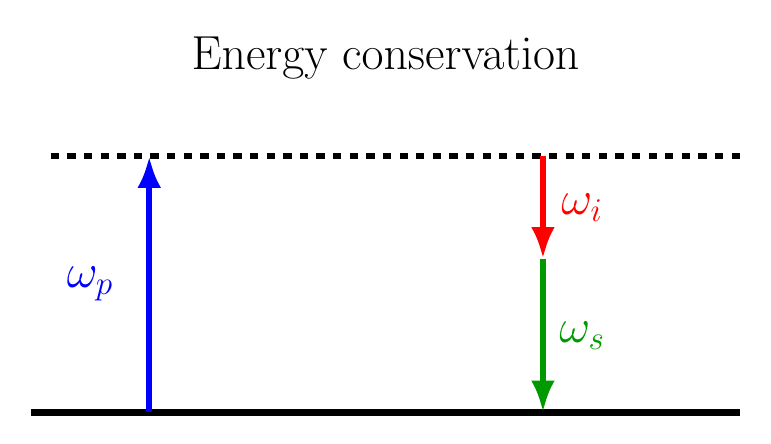
\begin{tikzpicture}
						%\useasboundingbox (0,0) rectangle (10,14);
						\tikzstyle{every node}=[font=\LARGE]
						
						\pgfmathsetmacro{\yTop}{12.5}
						\pgfmathsetmacro{\yBottom}{9.25}
						\pgfmathsetmacro{\yMid}{\yBottom + 0.6*(\yTop - \yBottom)}
						\pgfmathsetmacro{\pLab}{\yBottom + 0.5*(\yTop - \yBottom)}
						\pgfmathsetmacro{\sLab}{\yBottom + 0.3*(\yTop - \yBottom)}
						\pgfmathsetmacro{\iLab}{\yBottom + 0.8*(\yTop - \yBottom)}
						
						
						\draw [line width=2.5pt] (3.5,\yBottom) -- (12.5,\yBottom);
						\draw [ color={rgb,255:red,0; green,0; blue,255}, line width=2pt,-{Latex[length=4mm]}] (5,\yBottom) -- (5,\yTop);
						\draw [line width=2.3pt, dashed] (3.75,\yTop) -- (12.5,\yTop);
						\draw [ color={rgb,255:red,255; green,0; blue,0}, line width=2pt,-{Latex[length=4mm]}] (10,\yTop) -- (10,\yMid);
						\draw [ color=black!40!green, line width=2pt,-{Latex[length=4mm]}] (10,\yMid) -- (10,\yBottom);
						\node [font=\LARGE, color={rgb,255:red,0; green,0; blue,255}] at (4.25,\pLab) {$\omega_{\text{p}}$};
						\node [font=\LARGE, color={rgb,255:red,255; green,0; blue,0}] at (10.5,\iLab) {$\omega_{\text{i}}$};
						\node [font=\LARGE, color=black!40!green] at (10.5,\sLab) {$\omega_{\text{s}}$};
						
						\node [font=\LARGE] at (8,13.75) {Energy\,\,conservation};
						
						\end{tikzpicture}
					}%
			\end{center}
			%\vspace[2em]
			\begin{equation}
					\omega_{\text{p}} = \omega_{\text{s}} + \omega_{\text{i}}
				\nonumber
			\end{equation} 
		\end{minipage}
		\hfill
		\begin{minipage}{.4\textwidth}
			\begin{center}
				\resizebox{\textwidth}{!}{%
					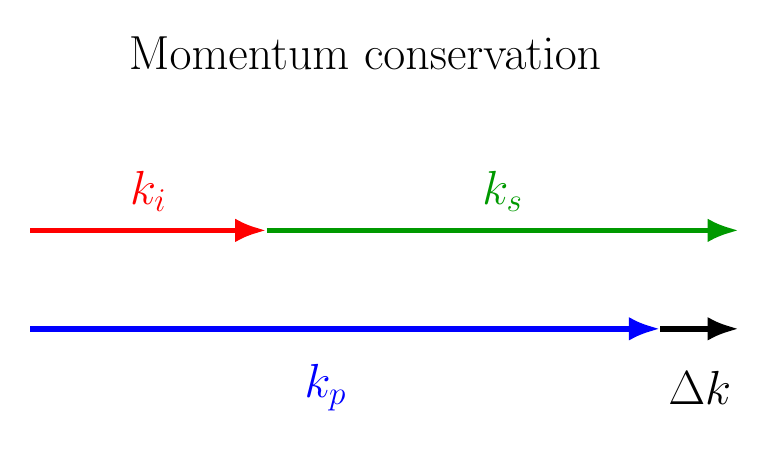
\begin{tikzpicture}
						%\useasboundingbox (0,0) rectangle (10,14);
						\tikzstyle{every node}=[font=\LARGE]
						\draw [ color={rgb,255:red,0; green,0; blue,255}, line 	width=2pt, -{Latex[length=4mm]}] (15,10.25) -- (23,10.25);
						\draw [ color={rgb,255:red,0; green,0; blue,0}, line width=2pt, 	-{Latex[length=4mm]}] (23,10.25) -- (24,10.25);
						\draw [ color={rgb,255:red,255; green,0; blue,0}, line 	width=2pt, -{Latex[length=4mm]}] (15,11.5) -- (18,11.5);
						\draw [ color=black!40!green, line width=2pt, 	-{Latex[length=4mm]}] (18,11.5) -- (24,11.5);
						
						\node [font=\LARGE, color={rgb,255:red,0; green,0; blue,255}] at 	(18.75,9.5) {$k_{\text{p}}$};
						\node [font=\LARGE, color={rgb,255:red,0; green,0; blue,0}] at 	(23.5,9.5) {$\Delta k$};
						\node [font=\LARGE, color={rgb,255:red,255; green,0; blue,0}] at 	(16.5,12) {$k_{\text{i}}$};
						\node [font=\LARGE, color=black!40!green] at (21,12) 	{$k_{\text{s}}$};
						
						
						\node [font=\LARGE] at (19.25,13.75) {Momentum\,\,conservation};
						
						% Coordinates
						\coordinate (A) at (7,6.5);
						\coordinate (B) at (10.5,6.5);
						%
						\coordinate (B') at (14.5,7);
						\coordinate (B'') at (14.5,6);
						\coordinate (C') at (18,7);
						\coordinate (C'') at (18,6);
			
				\end{tikzpicture}
				}%
			\end{center}
			%\vspace[2em]
			\begin{equation}
					\myvect{k}_{\text{p}} = \myvect{k}_{\text{s}} + 	\myvect{k}_{\text{i}} - 	\Delta \myvect{k}
				\nonumber
			\end{equation} 
		\end{minipage}
					
		\end{figure}
	\end{frame}
	
	\begin{frame}{Transmittance model}
		\begin{minipage}{.4\textwidth}
			\centering
			Conventional approach:
			\begin{equation}
				\begin{aligned}
					N_{\text{tot}}^{\text{ref}} &= \eta_{\text{idl}} \, N_{\mathrm{g}} 	+ N_{\text{noise}}^{\text{ref}} \\[0.5em]
					N_{\text{tot}}^{\text{sam}} &= T \, \eta_{\text{idl}} \, 	N_{\mathrm{g}} + N_{\text{noise}}^{\text{sam}}
				\end{aligned}
				\label{eq:SingleSam}
				\nonumber
			\end{equation}
		\end{minipage}
		\hfill
		\begin{minipage}{.4\textwidth}
			\centering
			Coincidence approach:
			\begin{equation}
				\begin{aligned}
					N_{\text{cc}}^{\text{pure,sam}} &= T \,\eta_{\text{idl}} \,\eta_{\text{sig}} \, N_{\mathrm{g}}, \\[0.5em]
					N_{\text{cc}}^{\text{pure,ref}} &= \eta_{\text{idl}} \,\eta_{\text{sig}} \, N_{\mathrm{g}}
				\end{aligned}
				\label{eq:pureCoinc}
				\nonumber
			\end{equation}
		\end{minipage}
	\end{frame}
	
	\begin{frame}{Conventional approach}
		\begin{minipage}{0.6\textwidth}
			\centering
			\only<1>{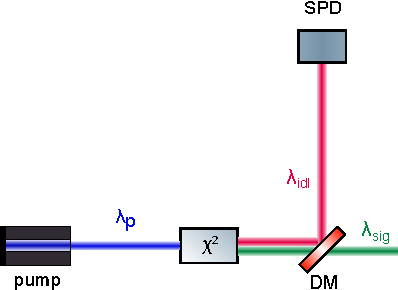
\includegraphics[width=.7\textwidth]{Images/ConventionalSetup_NoSam.pdf}}
			\only<2->{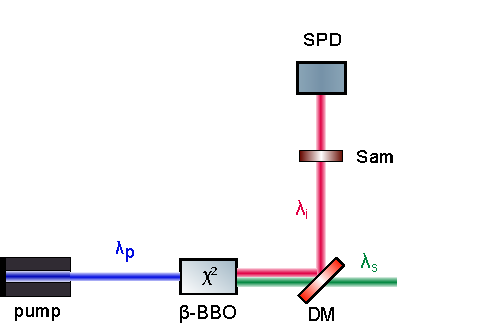
\includegraphics[width=.7\textwidth]{Images/ConventionalSetup.pdf}}
		\end{minipage}%
		\hfill
		\begin{minipage}{0.35\textwidth}
			\[
			\begin{aligned}
				\uncover<1->{N_{\text{tot}}^{\text{ref}} &= \eta_{\text{idl}} N_{\mathrm{g}} + N_{\text{noise}}^{\text{ref}}} \\[0.5em]
				\uncover<2->{N_{\text{tot}}^{\text{sam}} &= T\,\eta_{\text{idl}} N_{\mathrm{g}} + N_{\text{noise}}^{\text{sam}} } \\[1em]
				\uncover<3->{\Rightarrow T &= \frac{\,N_{\text{tot}}^{\text{sam}} - N_{\text{noise}}^{\text{sam}}\,}
				{\,N_{\text{tot}}^{\text{ref}} - N_{\text{noise}}^{\text{ref}}\,} }
			\end{aligned}
			\]
		\end{minipage}
	\end{frame}
		
	
	\begin{frame}{Coincidence approach}
		\begin{minipage}{.6\textwidth}
			\centering
			\only<1>{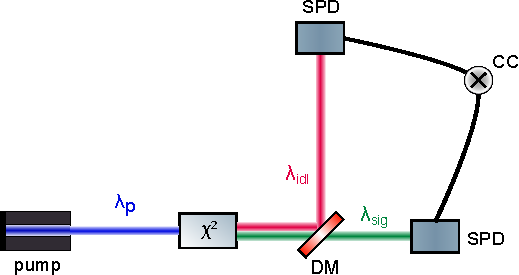
\includegraphics[width=.9\textwidth]{Images/CoincSetup_NoSam.pdf}}
			\only<2->{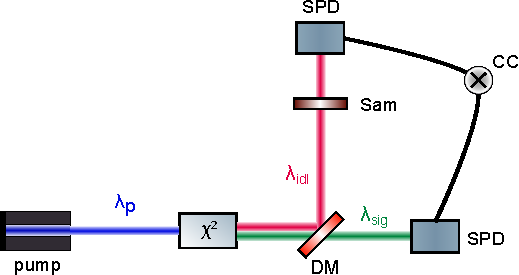
\includegraphics[width=.9\textwidth]{Images/CoincSetup_Sam.pdf}}
		\end{minipage}
		\hfill
		\begin{minipage}{.35\textwidth}
			\[
			\begin{aligned}
				\uncover<1->{N_{\text{cc,tot}}^{\text{ref}} &= \eta_{\text{idl}} \,\eta_{\text{sig}} \, N_{\mathrm{g}} + N_{\text{ac}}^{\text{ref}} } \\[1em]
				\uncover<2->{N_{\text{cc,tot}}^{\text{sam}} &= T \,\eta_{\text{idl}} \,\eta_{\text{sig}} \, N_{\mathrm{g}} + N_{\text{ac}}^{\text{sam}} } \\[1em]
				\uncover<3->{
				\Rightarrow T &= \frac{\,N_{\text{tot,cc}}^{\text{sam}} - N_{\text{ac}}^{\text{sam}}\,}{\,N_{\text{tot,cc}}^{\text{ref}} - N_{\text{ac}}^{\text{ref}}\,}
				} 
			\end{aligned}
			\]
		\end{minipage}
	\end{frame}
	
%	\begin{aligned}
%		\uncover<1->{N_{\text{cc,pure}}^{\text{ref}} &= \eta_{\text{idl}} \,\eta_{\text{sig}} \, N_{\mathrm{g}} \\[0.5em]
%			N_{\text{cc,tot}}^{\text{ref}} &= N_{\text{cc,pure}}^{\text{ref}} + N_{\text{ac}}^{\text{ref}} } \\[1em]
%		\uncover<2->{N_{\text{cc,pure}}^{\text{sam}} &= T \,\eta_{\text{idl}} \,\eta_{\text{sig}} \, N_{\mathrm{g}} \\[0.5em]
%			N_{\text{cc,tot}}^{\text{sam}} &= N_{\text{cc,pure}}^{\text{sam}} + N_{\text{ac}}^{\text{sam}} } \\[1em]
%		\uncover<3->{
%			\Rightarrow T &= \frac{\,N_{\text{tot,cc}}^{\text{sam}} - N_{\text{ac}}^{\text{sam}}\,}{\,N_{\text{tot,cc}}^{\text{ref}} - N_{\text{ac}}^{\text{ref}}\,}
%		} 
%	\end{aligned}
	
	\begin{frame}{Transmittance model}
		\begin{Block}{Conventional approach:}
			\resizebox{\textwidth}{!}{$
				\operatorname{Var}(T) 
				= \left( \frac{1}{\eta_{\text{idl}}\,N_{\mathrm{g}}} \right)^{2}
				\Bigg[
				\textcolor<2->{red}{\operatorname{Var}\!\left(N_{\text{tot}}^{\text{sam}}\right)} 
				+ \textcolor<2->{red}{\operatorname{Var}\!\left(N_{\text{noise}}^{\text{sam}}\right)} 
				+ T^{2} \Big[ 
				\textcolor<2->{red}{\operatorname{Var}\!\left(N_{\text{tot}}^{\text{ref}}\right)} 
				+ \textcolor<2->{red}{\operatorname{Var}\!\left(N_{\text{noise}}^{\text{ref}}\right) }
				\Big]
				\Bigg]
			$}
		\end{Block}
		%\vspace{2em}
		\begin{Block}{Coincidence approach:}
			\resizebox{\textwidth}{!}{$
				\operatorname{Var}(T) 
				= \left( \frac{1}{\eta_{\text{sig}}\,\eta_{\text{idl}}\,N_{\mathrm{g}}} \right)^{2}
				\Bigg[
				\textcolor<2>{red}{\operatorname{Var}\!\left(N_{\text{tot,cc}}^{\text{sam}}\right) }
				+ \textcolor<2>{red}{\operatorname{Var}\!\left(N_{\text{ac}}^{\text{sam}}\right) }
				+ T^{2} \Big[ 
				\textcolor<2>{red}{\operatorname{Var}\!\left(N_{\text{tot,cc}}^{\text{ref}}\right) }
				+ \textcolor<2>{red}{\operatorname{Var}\!\left(N_{\text{ac}}^{\text{ref}}\right) }
				\Big]
				\Bigg]
			$}
		\end{Block}
	\end{frame}
	
	
	\section{Experiment}
	\begin{frame}{Experimental setup}
			\begin{center}
				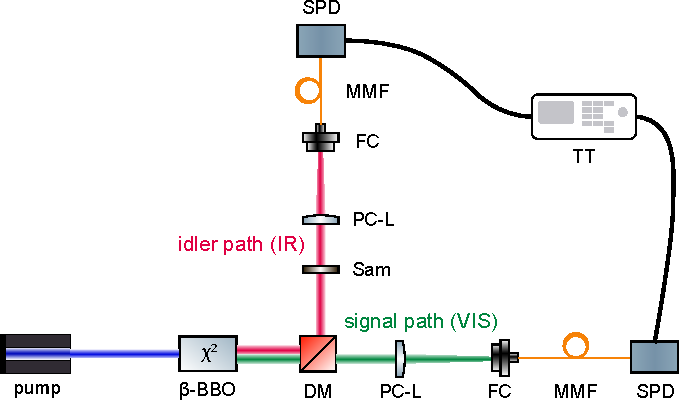
\includegraphics[width=.7\textwidth]{Images/DupishSetup.pdf}
			\end{center}
			
	\end{frame}
	\section{Results}
	
	\begin{frame}{Dark counts}
		\begin{minipage}{.45\textwidth}
			\centering
			\textbf{Idler arm}
			\vspace{2em}
			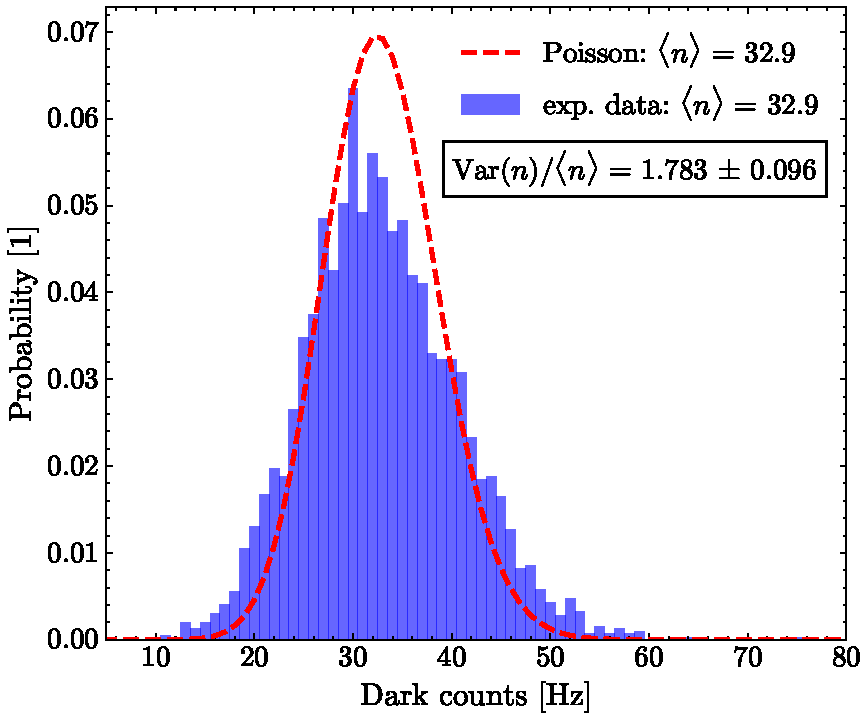
\includegraphics[width=\textwidth]{Images/DC_Idl_2.pdf}
		\end{minipage}
		\hfill
		\begin{minipage}{.45\textwidth}
			\centering
			Signal arm
			\vspace{2em}
			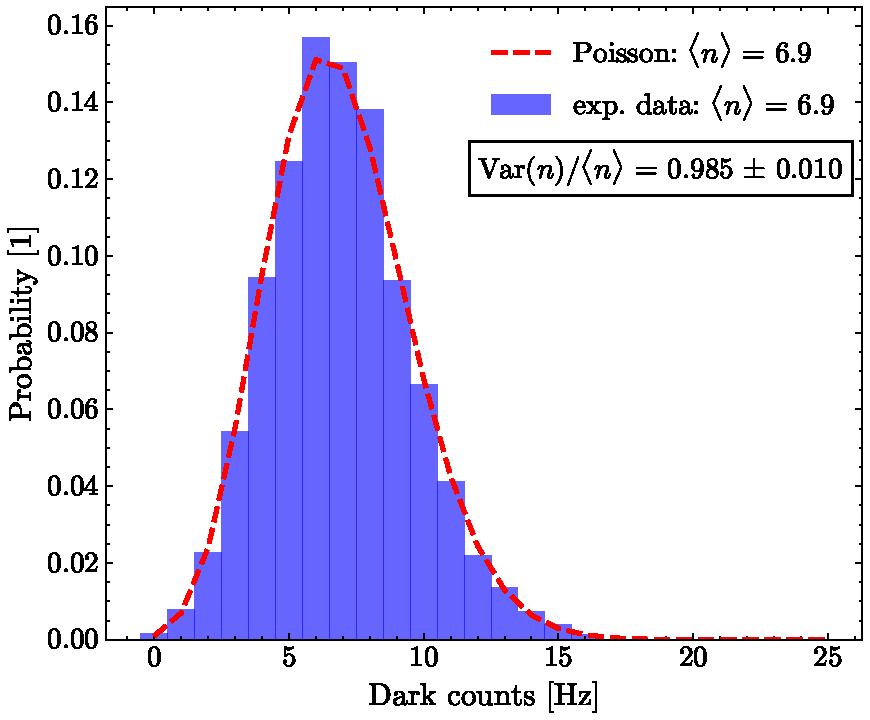
\includegraphics[width=\textwidth]{Images/DC_Sig_2.pdf}
		\end{minipage}
	\end{frame}
	
	\begin{frame}{Single counts}
		\begin{minipage}{.5\textwidth}
			\centering
			\textbf{Idler arm}
			\vspace{2em}
			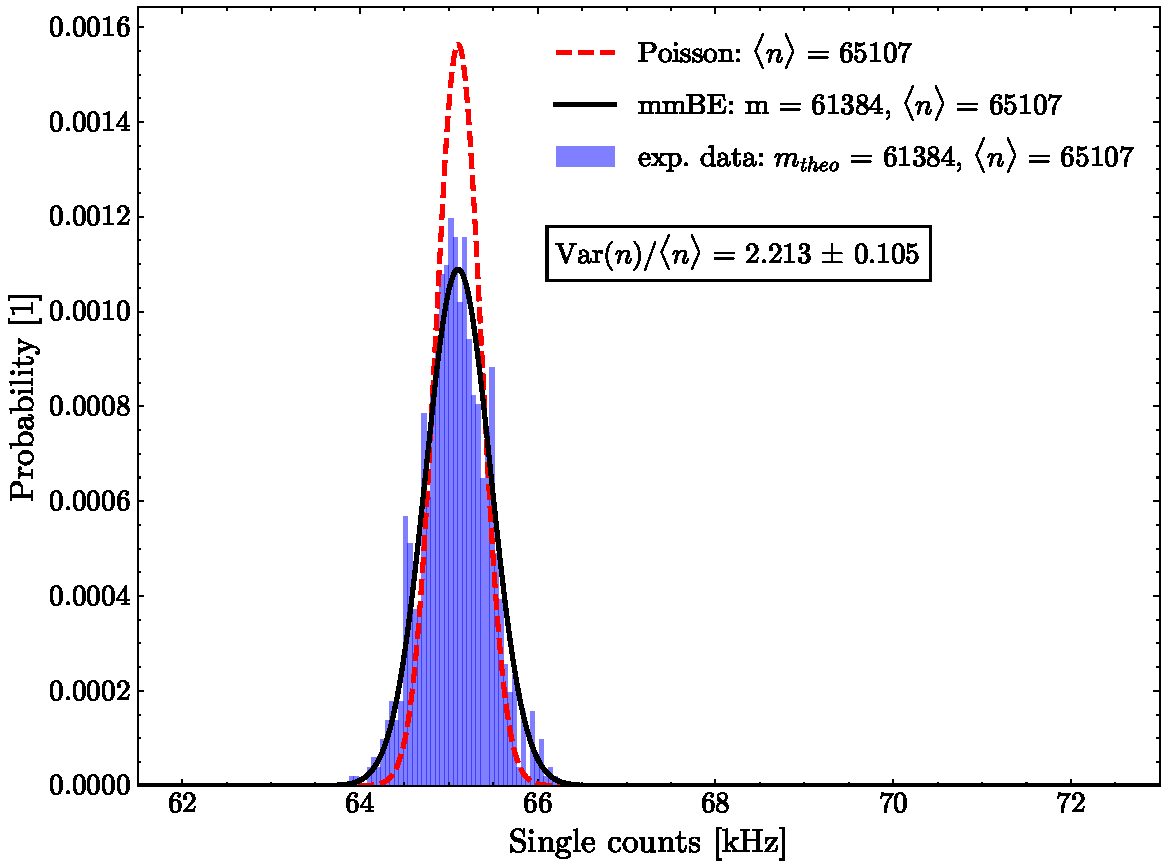
\includegraphics[width=\textwidth]{Images/SingleStatisticsIdler.pdf}
		\end{minipage}
		\hfill
		\begin{minipage}{.5\textwidth}
			\centering
			Signal arm
			\vspace{2em}
			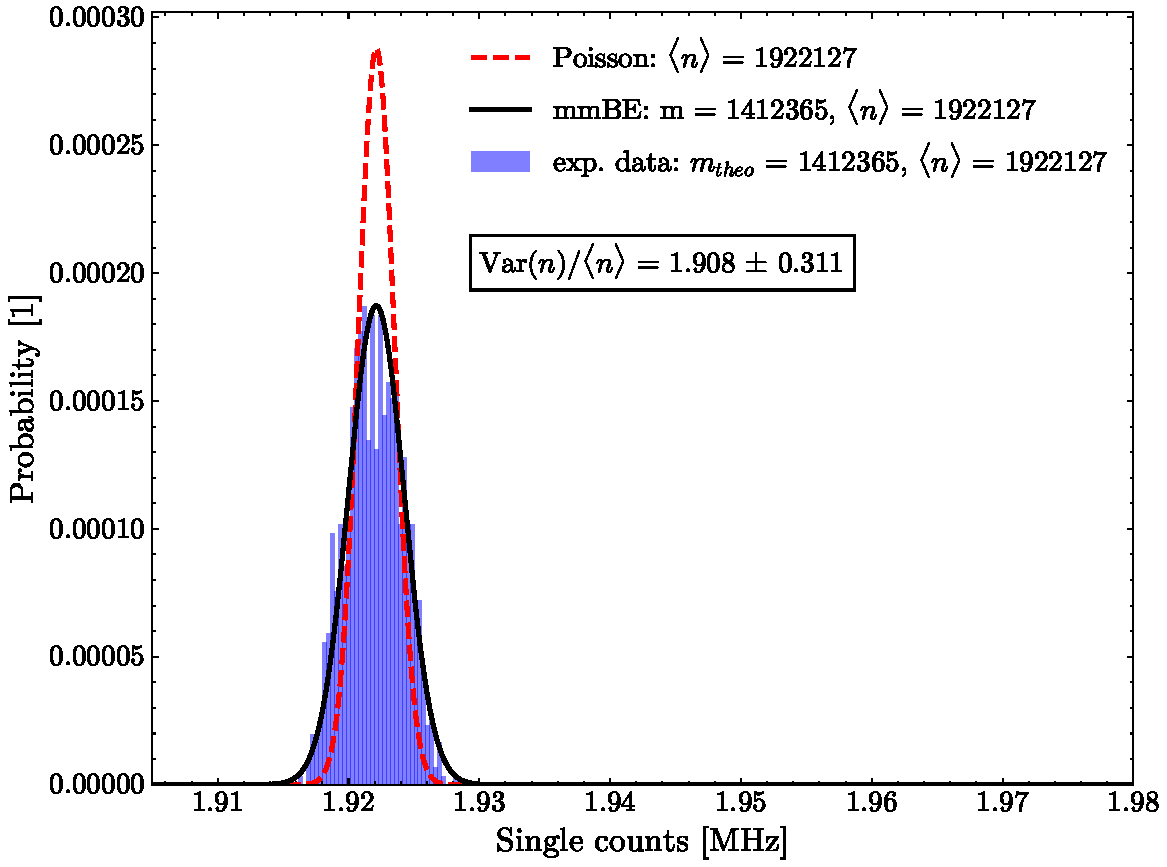
\includegraphics[width=\textwidth]{Images/SingleStatisticsSignal.pdf}
		\end{minipage}
	\end{frame}
	
	
	
	
	\begin{frame}{Slide title in Palatino Linotype Font}
		\begin{block}{block environment (lower-case b)}
			itemize:
			\begin{itemize}
				\item First Level
				\begin{itemize}
					\item Second Level
					\begin{itemize}
						\item Third Level has no item mark
					\end{itemize}
				\end{itemize}
			\end{itemize}
		\end{block}
		\begin{Block}{Block environment (upper-case B)}
		enumerate:
		\begin{enumerate}
			\item First Level
			\begin{enumerate}
				\item Second Level
				\begin{enumerate}
					\item Third Level
				\end{enumerate}
			\end{enumerate}
		\end{enumerate}
		\end{Block}
	\end{frame}
	
	\section{Simulation}
	\begin{frame}{Font types}
		\begin{table}
			\begin{tabular}{ll}
				Normal & Lorem ipsum dolor sit amet, consectetur adipiscing elit.\\
				\textbf{Bold} & \textbf{Lorem ipsum dolor sit amet, consectetur adipiscing elit.}\\
				\textit{Italic} & \textit{Lorem ipsum dolor sit amet, consectetur adipiscing elit.}\\
				\textbf{\textit{BoldItalic}} & \textbf{\textit{Lorem ipsum dolor sit amet, consectetur adipiscing elit.}}
			\end{tabular}
		\end{table}
		\begin{equation}
			\textrm{e}^{\textrm{i}\pi}+1=0
			\label{eq1}
		\end{equation}
		Equations like eq.~\eqref{eq1} use the beamer default font computer modern.
	\end{frame}
	
	\section{Summary}
	\begin{frame}{Summary and Outlook}
		\begin{Block}{Git repository}
			public accessible:\\
			{\scriptsize\url{https://git.tpi.uni-jena.de/mstnhsr/latexbeamer_corporatedesign}}
		\end{Block}
		\begin{Block}{Feedback}
			marc.steinhauser@uni-jena.de
		\end{Block}
	\end{frame}
	
\end{document}
 
